%!TEX root = ..\..\main.tex
\chapter{Maximum Likelihood Location Mixtures}
\label{Ch:Mixtures}

\lhead{Chapter \ref{Ch:Mixtures}. \emph{Maximum Likelihood Location Mixtures}}

\graphicspath{{Figures/Mixtures/}}

%-------------------------------------------------------------------------------
%	Chapter Text
%-------------------------------------------------------------------------------

\section{Introduction}
	Mixtures of distributions have been used to model a wide variety of phenomena, with successful applications in the fields of ``astronomy, biology, genetics, medicine, psychiatry, economics, engineering, and marketing, among many other fields in the biological, physical, and social sciences'' \cite[Section 1.1.1]{McLachlan2004-ik}. Mixture models have been in use for over 100 years. In 1984, Pearson used a mixture of two normal densities to model the distribution of the ratio of forehead to body lengths of a sample of 1000 crabs \cite{Pearson1894-qv}. His mixture of two normals was able to account for the skewness in the data, which a single normal could not model. Pearson suggested that this signalled the existence of two sub-populations of crabs; each associated with its own normal distribution.

	However, we do not require that data comes from a mixture of distributions in any physical sense for mixtures to be a useful modelling tool. 
	One of the traits that has contributed to the extent of the use of mixtures is that they provide a convenient semi-parametric way of modelling unknown distributions. They are particularly useful in situations where a parametric method is too restrictive to satisfactorily model the data, and a fully non-parametric method, such as kernel density estimation, may require evaluating a sum which contains more terms than desired. By way of illustration, Priebe in \cite{Priebe1994-ng} discussed modelling a log normal density using a mixture of normals. With $n = 10000$ observations, Priebe only required about 30 normals to obtain a good approximation. This is in contrast to a kernel density estimator which in this case would be essentially a mixture of 10000 normals.

	[WHAT ELSE?]

	\subsection{Definitions}
	A \emph{mixture density} is a probability density function that can be written in the form
	\begin{equation}
		f_Q(\vect{x}) = \int_\Omega f(\vect{x}; \vect{\theta}) \intd Q(\vect{\theta})
		\label{eq:mixture definition}
	\end{equation}
	where $f(\vect{x};\vect{\theta})$ is the \emph{component density}, parametrised by $\vect{\theta} \in \Omega$, and $Q$ is a probability distribution on $\Omega$, called the \emph{mixing distribution}. In the case that $Q$ is a discrete probability distribution, with probability masses $p_j$ at points $\vect{\theta}_j$, $j = 1, \dots, m$, the mixture density in \eqref{eq:mixture definition} is a \emph{finite mixture} and can be written
	\begin{equation}
		f_Q(\vect{x}) = f_{\vect{\theta}, \vect{p}}(\vect{x}) = \sum_{j = 1}^m p_j f(\vect{x}; \vect{\theta}_j).
	\end{equation}

	In this chapter, we will be concerned only with finite mixtures on the real line, whose component densities are parametrised by a single shifting parameter, $\theta$. This is what we will call a \emph{location mixture}, and it can be written as
	\begin{equation}
		f_{\vect{p}, \vect{\theta}} = \sum_{j = 1}^m p_j f(x - \theta_j).
		% \label{eq:mixturesum}
	\end{equation}
	Looking only at mixtures of this form is not as restrictive as it may at first seem. Using a finite location mixture of normals, you can approximate any continuous density arbitrarily well [BETTER CITATION] \cite{McLachlan2004-ik}.

	A common question when using mixtures is the following. Let $\vect{X} = (X_1, \dots, X_n)$ be a random sample of size $n$, where $X_i$ has probability density function $g(\vect{x})$. Given $\vect{x} = (x_1, \dots, x_n)$, an observed random sample of $\vect{X}$, and a component density $f(\vect{x}; \vect{\theta})$, how do we choose the mixing distribution $Q$ so that $f_Q(\vect{x})$ is a good approximation for $g(\vect{x})$?

	One answer to this question is to use maximum likelihood.

	[UP TO HERE]
	% History, background, usefulness
	% Definitions
	% Log likelihood
	% Location mixtures


	A location mixture on $\mathbb{R}$ with mixing distribution $Q$ and component density $f(x)$ can be written as
	\begin{equation}
		f_Q(x) = \int_{-\infty}^\infty f(x-\theta) \intd Q(\theta).
	\label{eq:mixtureint}
	\end{equation}

	Given a sample $\vect{x} = (x_1,\dots,x_n)$, we wish to find a distribution that maximizes the log likelihood	
	\begin{equation}
		L(Q;\vect{x}) = \sum_{i = 1}^n \log(f_Q(x_i)).
	\label{eq:loglikelihood}
	\end{equation}
	Lindsay showed that under quite general conditions, such a maximizing distribution exists and has no more than $n$ points of support \cite{Lindsay1983-tf}. It is therefore common to use
	\begin{equation}
		f_{\vect{p},\vect{\theta}}(x) = \sum_{j = 1}^m p_j f(x - \theta_j)
	\label{eq:mixturesum}
	\end{equation}
	instead of \eqref{eq:mixtureint} as our definition of a location mixture. We note that \eqref{eq:mixtureint} is equivalent to \eqref{eq:mixturesum} in the case where $Q$ is a discrete distribution which places probability masses of weight $p_j$ at locations $\theta_j$, for $j = 1,\dots,m$. The order of the $x_i$ does not matter and so we will assume without loss of generality that $x_1 \leq x_2 \leq \dots \leq x_n$ throughout.
	
	In this paper we are primarily interested in the number of probability masses that are required in the maximizing mixture. We will call this quantity $K_{\vect{x}}$. It should be noted that there is not always a unique mixing distribution that maximizes \eqref{eq:loglikelihood}. However we can choose $K_{\vect{x}}$ to be the smallest number of probability masses that any of the maximizing distributions have.

\section{Numerical Results}
		One point which we wish to emphasize is that, given a component density $f$, $K$ is a function of $\vect{x}$ only. We can visualise this for small values of $n$. In Figure \ref{fig:n3phase}, we empirically found the MLE for $\vect{x} = (0,x_2,x_3)$ and recorded the number of probability masses in the maximizing mixture. We took values for $x_2$ and $x_3$ from an evenly spaced grid with $-6\leq x_2,x_3\leq 6$. We fixed $x_1 = 0$ since the shape of the maximum likelihood mixture (and therefore $K_{\vect{x}}$) depends only on the relative location of the $x_i$, not their absolute location.
		
		\begin{figure}[ht]
			\centering
			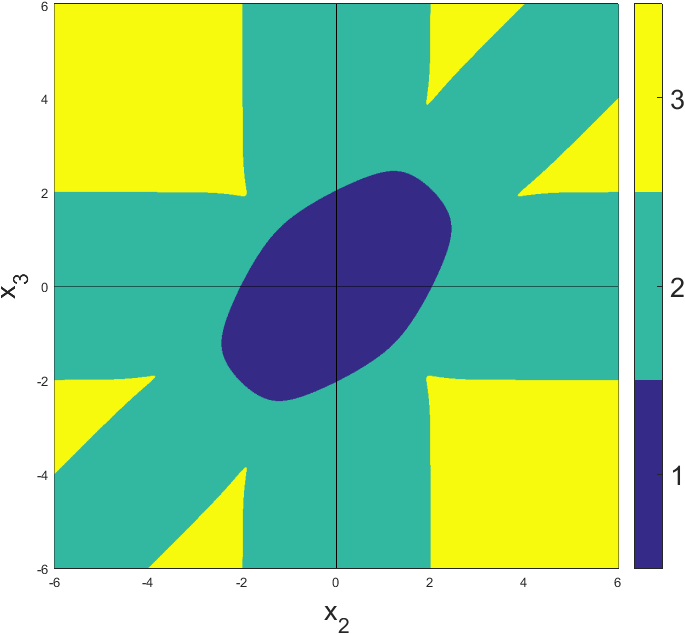
\includegraphics[width=0.8\textwidth]{Sigma1n3res1024width6}
			\caption{$K$ as a function of $x_2$ and $x_3$ (with $x_1 = 0$) for a normal component density with unit variance.}\label{fig:n3phase}
		\end{figure}
		
		For a particular choice of component density, we can partition $\mathbb{R}^n$ into sets 
		\begin{equation}
			C_k = \{ \vect{x} \in \mathbb{R}^n | K_{\vect{x}} = k \}, \hspace{40pt} k = 1,\dots,n.
		\end{equation}
		The problem of determining $K_{\vect{x}}$ is then the same as determining in which of the $C_k$ $\vect{x}$ lies.

	\subsection{Motivating Example}

\section{Summary of Lindsay}

\section{Results for \texorpdfstring{$n = 2$}{n = 2}}
	In this section, we present Theorem \ref{thm:n=2 inflection result} which 
	expands upon the results found in \cite{Lindsay1983-tf} and \cite{Lindsay1983a-he}.

	\subsection{Things that are referenced}
	REWORK CONTENTS OF THIS SUBSECTION INTO MAIN TEXT.
	\begin{equation}
		M(\vect{u}) = \sum_{i=1}^n \log(u_i)
		\label{eq:transformedlikelihood}
	\end{equation}

	\begin{theorem}
		If $\Gamma$ is compact then there exists a unique point on the boundary of $\conv(\Gamma)$ which maximizes the likelihood. This point corresponds to a distribution $Q$ which maximizes the likelihood and that has no more than $n$ point masses.
		\label{thm:LindsayGamma}
	\end{theorem}

	\subsection{The likelihood curve}
		In \cite{Lindsay1983-tf}, the problem of mixture likelihoods was looked at from a geometrical perspective. One key construction introduced by Lindsay was the \emph{likelihood curve},
		\begin{equation}
			\vect{\gamma}(\theta;\vect{x}) = (f(x_{1}-\theta),\dots,f(x_{n}-\theta))
			\label{eq:Gamma}
		\end{equation}
		and it's trace,
		\begin{equation}
			\Gamma_{\vect{x}} = \{\vect{\gamma}(\theta;\vect{x})| \theta \in \mathbb{R}\}.
		\end{equation}
		A useful property of the likelihood curve is that any convex combination of elements from $\Gamma_{\vect{x}}$ can be written as
		\begin{equation}
			\vect{u}(\vect{p},\vect{\theta};\vect{x}) = (f_{\vect{p},\vect{\theta}}(x_{1}),\dots,f_{\vect{p},\vect{\theta}}(x_{n})) = \sum_{j = 1}^m p_j \vect{\gamma}(\theta_j;\vect{x}), \hspace{30pt} \sum_{j=1}^m p_j = 1
			\label{eq:convexcombinationgamma}
		\end{equation}
		where $f_{\vect{p},\vect{\theta}}(x)$ is as defined in \eqref{eq:mixturesum}. The log likelihood of the corresponding distribution is simply the sum of the log of the components of $\vect{u}(\vect{p},\vect{\theta};\vect{x})$.
		
		One of Lindsay's main results, which follows from this observation, was that if
		\begin{equation}
			\hat{\vect{u}} = \argmax_{\vect{u} \in \conv(\Gamma_{\vect{x}})} \sum_{i=1}^n \log(u_i)
			\label{eq:optimalu}
		\end{equation}
		% where
		% \begin{equation}
		% 	U =  %\{\vect{u}(\vect{p},\vect{\theta};\vect{x}) |  \}
		% \end{equation}
		then we can write
		\begin{equation}
			\hat{\vect{u}} = \vect{u}(\vect{p},\vect{\theta};\vect{x})
		\end{equation}
		for some $\vect{p}$ and $\vect{\theta}$ whose dimension is no more than $n$. Furthermore, the corresponding distribution that places masses $p_j$ at locations $\theta_j$ maximizes \eqref{eq:loglikelihood}. There are some minor conditions on this result, but they will not cause any problems for our purposes and so will not be discussed (see \cite{Lindsay1983-tf} for details).
	\subsubsection{An example}
		\label{sec:mixturelikelihoods:example}
		The following example illustrates the geometrical approach given above. We consider the case where $n = 2$. Our sample is made up of two points, $X_1 = 1$ and $X_2 = 2$. We define
		\begin{equation}
		f_\theta(x) = \frac{1}{0.45 \sqrt{2 \pi}} \exp\left(-\frac{(x-\theta)^2}{2\cdot 0.45^2}\right)
		\end{equation}
		(i.e. a normal density with mean $\theta$ and variance $\sigma^2 = 0.45^2$) to be our component density.
		We trace out the set $\Gamma$ in Figure \ref{fig:TracingGamma}. 

		\begin{figure}[ht]
			\centering
			\begin{minipage}[b]{0.3\linewidth}
				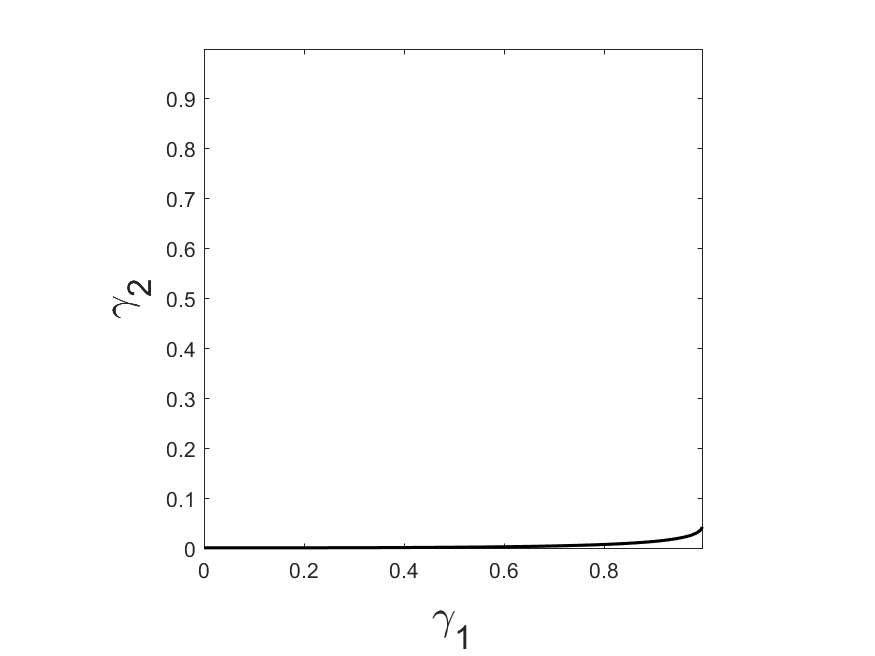
\includegraphics[width=\textwidth]{GammaTrace01}
			\end{minipage}
			\begin{minipage}[b]{0.3\linewidth}
				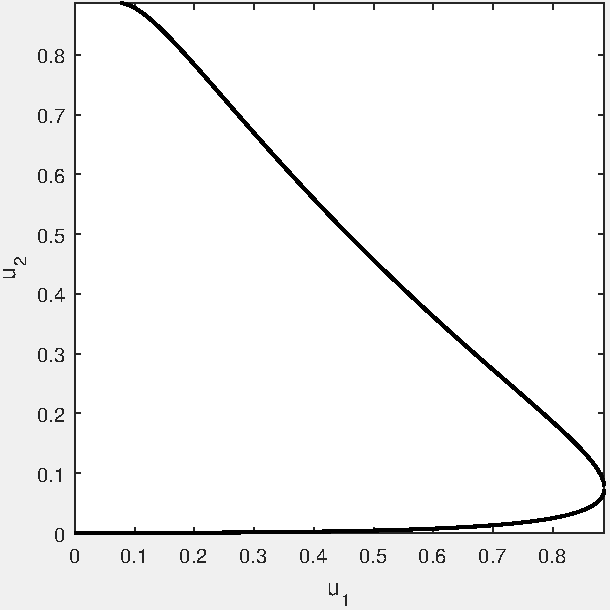
\includegraphics[width=\textwidth]{GammaTrace02}
			\end{minipage}
			\begin{minipage}[b]{0.3\linewidth}
				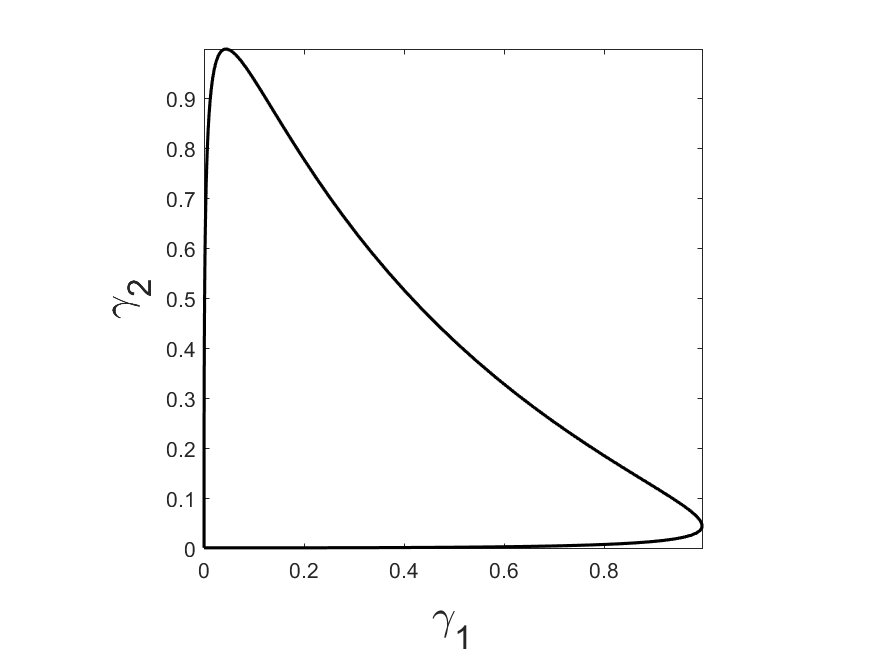
\includegraphics[width=\textwidth]{GammaTrace03}
			\end{minipage}
			\begin{minipage}[b]{0.3\linewidth}
				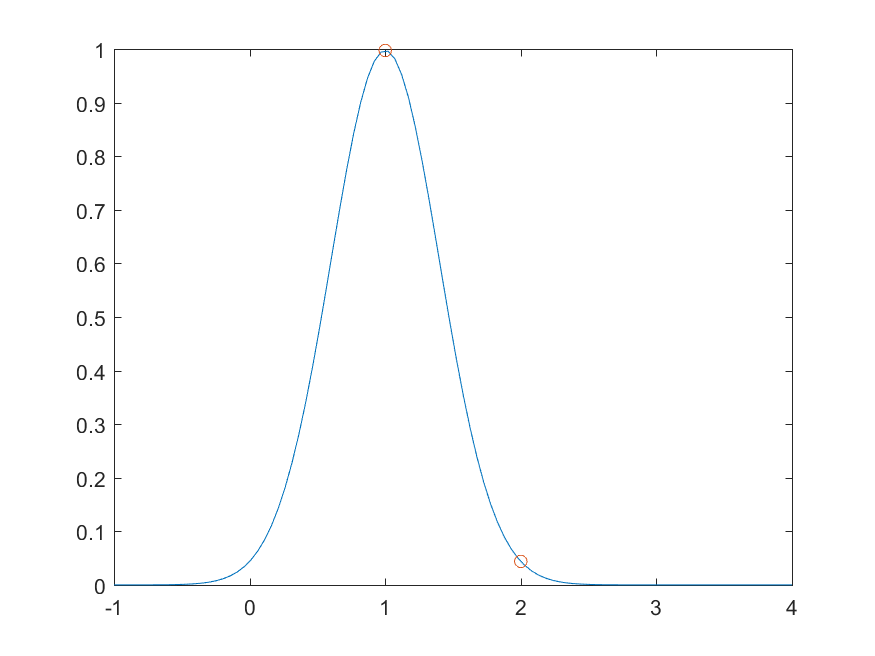
\includegraphics[width=\textwidth]{GammaTraceDensity01}
				\subcaption{$\theta = 1$}
			\end{minipage}
			\begin{minipage}[b]{0.3\linewidth}
				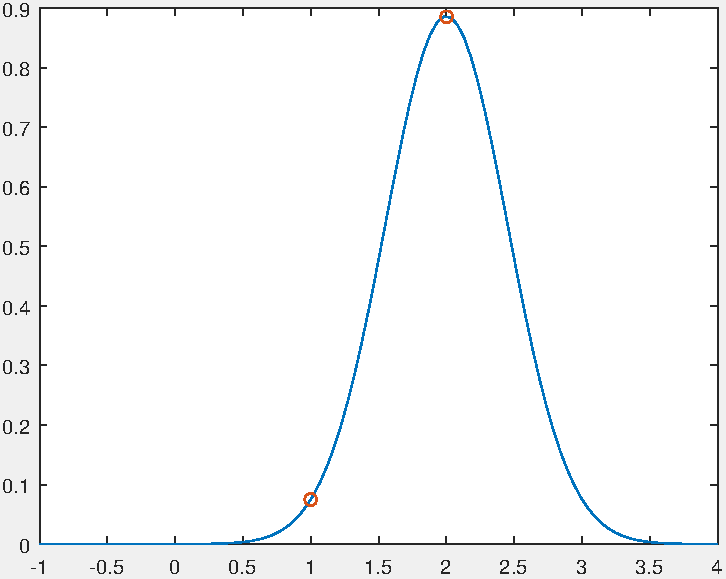
\includegraphics[width=\textwidth]{GammaTraceDensity02}
				\subcaption{$\theta = 2$}
			\end{minipage}
			\begin{minipage}[b]{0.3\linewidth}
				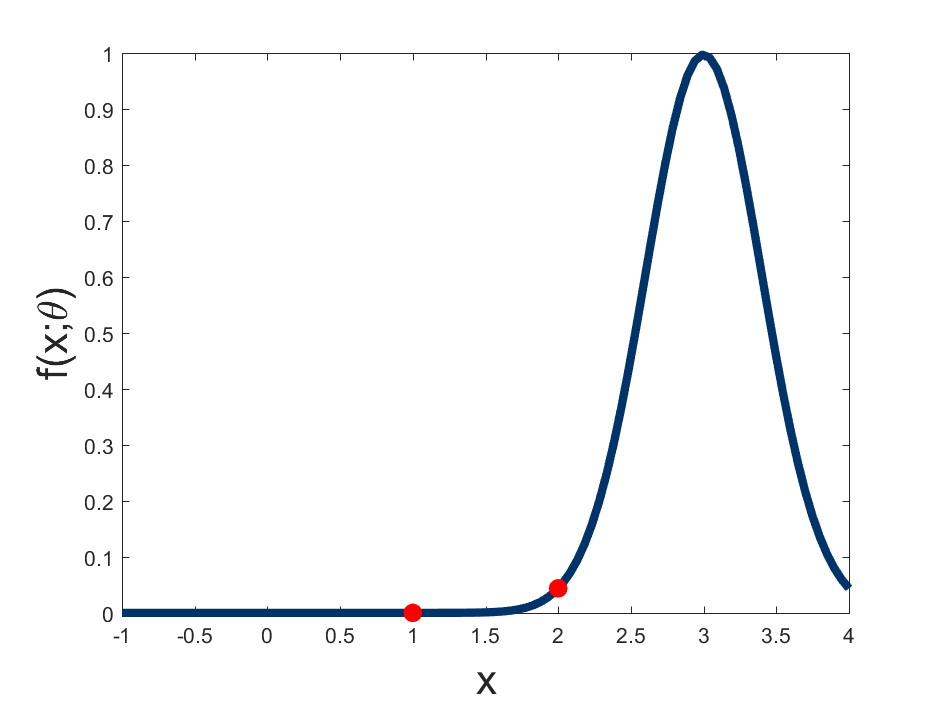
\includegraphics[width=\textwidth]{GammaTraceDensity03}
				\subcaption{$\theta = 3$}
			\end{minipage}
			\caption{The blue density is $f_\theta$ for $\theta = 1,2,3$. Each value of $\theta$ contributes a point to $\Gamma$ whose coordinates are given by $(f_\theta(X_1),f_\theta(X_2))$ (represented by the red circles). As we increase $\theta$ from $-\infty$ to $\infty$ we trace out more of $\Gamma$ (shown above).}\label{fig:TracingGamma}
		\end{figure}

		Note that while $\Gamma$ is bounded, it is not closed (it does not contain the limit point $(0,0)$), and so $\Gamma$ is not compact (as required by Theorem \ref{thm:LindsayGamma}). In fact, any positive density whose support is the whole real line will not contain the limit point $\vect{0}$ (where $\vect{0}$ represents the zero vector in $\mathbb{R}^n$). However, since $\vect{0}$ is clearly not going to be a part of a maximizing mixture, we are safe to apply Theorem \ref{thm:LindsayGamma} if $\Gamma \cup \{ \vect{0} \}$ is compact.

		%and so we will provide a slightly more general form of Theorem \ref{thm:LindsayGamma}.
		%\begin{theorem}
		%	Write $\vect{0}$ for the zero vector in $\mathbb{R}^n$. If $\Gamma \cup \{ \vect{0} \}$ is compact then there exists a unique point on the boundary of $\conv(\Gamma)$ which maximizes the likelihood. This point corresponds to a distribution $Q$ which maximizes the likelihood and that has no more than $n$ point masses.
		%\end{theorem}
		%\begin{proof}
		%	We need to show that $\vect{0}$ does not appear in the maximizing mixture. Clearly, $\vect{0}$ is not going to be a maximizing point.
		%\end{proof}

		We trace the boundary of $\conv(\Gamma)$ in Figure \ref{fig:GammaSol} along with a heat map of the objective function \eqref{eq:transformedlikelihood}.
		\begin{figure}[ht]
			\centering
			\begin{minipage}{0.4\textwidth}
				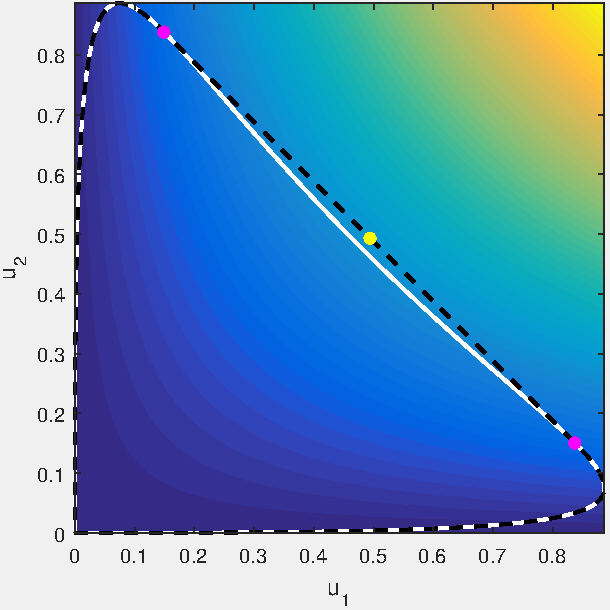
\includegraphics[width = \textwidth]{GammaOptimHullSol}
				\subcaption{}\label{fig:GammaSol:subfig:Gamma}
			\end{minipage}
			\begin{minipage}{0.5\textwidth}
				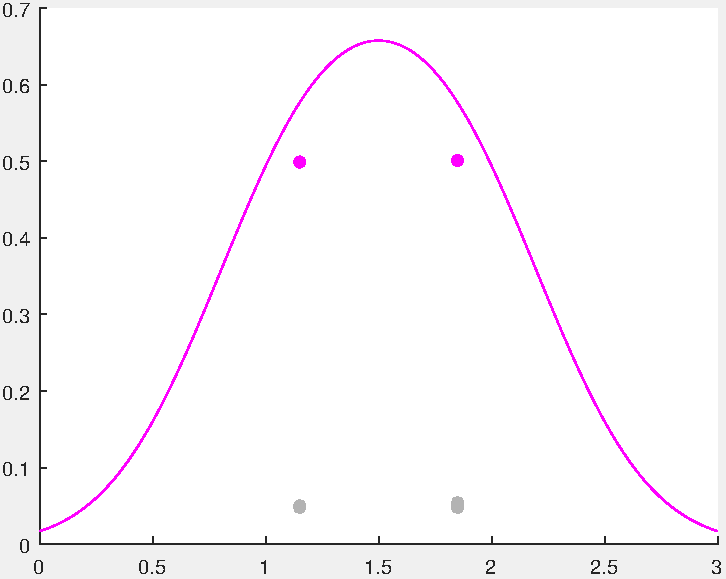
\includegraphics[width = \textwidth]{MixingSolSigma045}				\subcaption{}\label{fig:GammaSol:subfig:Density}
			\end{minipage}
			\caption{In (\subref{fig:GammaSol:subfig:Gamma}), the boundary of $\conv(\Gamma)$ is shown as a dashed black line, $\Gamma$ is the white curve, the heat map  shows the objective function (likelihood increases from blue to yellow) and the yellow point is the maximizing point which can be written as the convex combination of the two magenta points. These two magenta points correspond to the two probability masses in the maximizing mixing distribution (\subref{fig:GammaSol:subfig:Density}).}
			\label{fig:GammaSol}
		\end{figure}
		The optimal point is on the boundary of $\conv(\Gamma)$ as expected and it can be written as the  $p_1 \vect{f}(\theta_1) + p_2 \vect{f}(\theta_2)$ (where $p_1 + p_2 =1 $). These two points correspond to the two probability masses in the maximizing mixture distribution shown in Figure \ref{fig:GammaSol:subfig:Density}. These masses are located at $\theta_1$ and $\theta_2$ with weights $p_1$ and $p_2$.

	\subsection{The likelihood curve for \texorpdfstring{$n = 2$}{n = 2}}
		The shape of $\Gamma_\vect{x}$ can provide us with some insight into the behaviour of $K_\vect{x}$. In Figure \ref{fig:Gammaexample}, we give some examples of $\Gamma_\vect{x}$ for $n=2$ using a normal component density with variance $\sigma^2 = 1$. 
		\begin{figure}[ht]
			\begin{subfigure}[t]{0.32\textwidth}
				\centering
				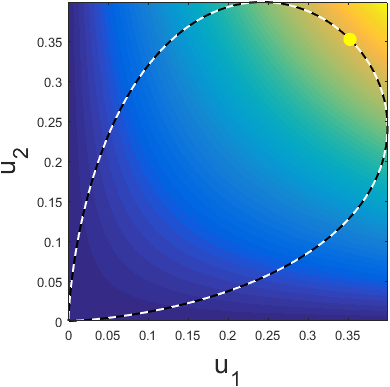
\includegraphics[width = \textwidth]{Sigma1x1_0-x2_1}
				\caption{$\vect{x} = (0,1)$} \label{subfig:gammaexamplea}
			\end{subfigure}
			\begin{subfigure}[t]{0.32\textwidth}
				\centering
				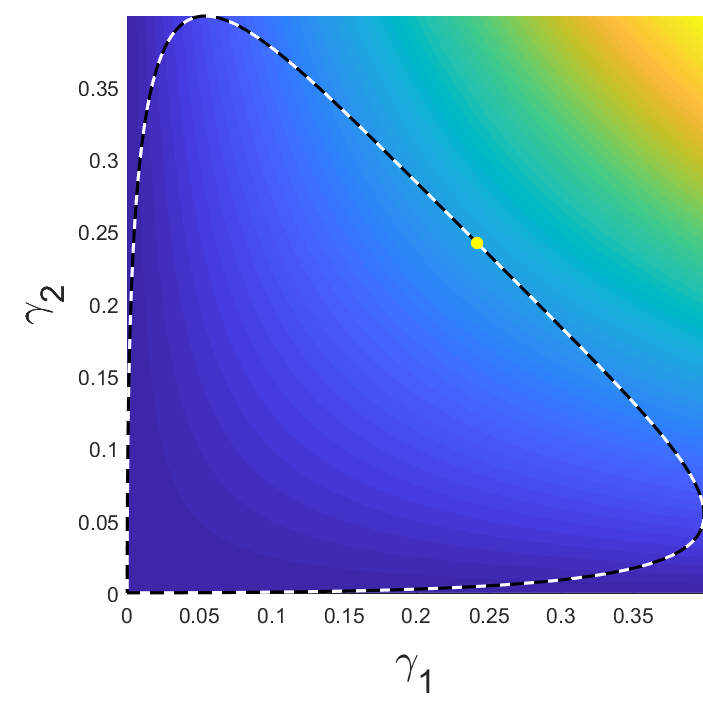
\includegraphics[width = \textwidth]{Sigma1x1_0-x2_2}
				\caption{$\vect{x} = (0,2)$} \label{subfig:gammaexampleb}
			\end{subfigure}
			\begin{subfigure}[t]{0.32\textwidth}
				\centering
				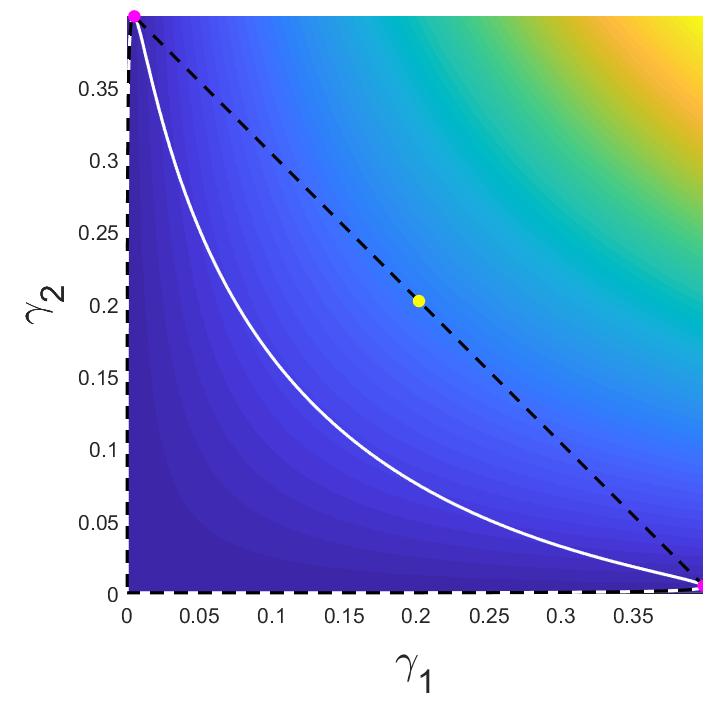
\includegraphics[width = \textwidth]{Sigma1x1_0-x2_3}
				\caption{$\vect{x} = (0,3)$} \label{subfig:gammaexamplec}
			\end{subfigure}
			\caption{The curve $\Gamma_\vect{x}$ for three different $\vect{x}$ along with the boundary of $\conv(\Gamma_\vect{x})$. The objective function from \eqref{eq:optimalu} is represented as a heat map. The optimal point $\hat{\vect{u}}$ is shown in yellow, and where applicable, the points $\vect{\gamma}(\theta_j)$ that make up $\hat{\vect{u}}$ (as in \eqref{eq:convexcombinationgamma}) are shown in magenta.}
			\label{fig:Gammaexample}
		\end{figure}
		In particular, we note that the distance between $x_1$ and $x_2$ has a strong effect on the shape of $\Gamma_\vect{x}$. In Figure \ref{subfig:gammaexamplea}, the points are distance 1 apart and $\Gamma_\vect{x}$ is the boundary of $\conv(\Gamma_\vect{x})$. In this case, it is clear that $K_\vect{x} = 1$. In Figure \ref{subfig:gammaexamplec}, the points are distance 3 apart and the optimal point no longer lies on $\Gamma_\vect{x}$. This results in the maximum likelihood mixing distribution needing two points of support and so $K_\vect{x} = 2$. The boundary case, where $\Gamma_\vect{x}$ goes from being a convex curve to having the indentation shown in Figure \ref{subfig:gammaexamplec}, is shown in Figure \ref{subfig:gammaexampleb}.

		Obtaining results about where these boundaries lie is very difficult in higher dimensions. In \cite{Lindsay1983a-he}, Lindsay used the sign of the curvature of $\vect{\gamma}(\theta;\vect{x})$ to obtain results for $n=2$ when the component density is in the exponential family. Here we will present an extension to Lindsay's results by considering densities that satisfy the following assumptions.
	
		\begin{assumption}[Continuity]
			$f(x)$ is a continuous density and has the whole real line as its support.
			\label{assump:reallinesupport}
		\end{assumption}
		
		\begin{assumption}[Differentiability]
			$f(x)$ is twice differentiable.
			\label{assump:twicediff}
		\end{assumption}
		
		\begin{assumption}[Unimodality]
			$f(x)$ has a single mode at $x=0$. I.e. $f'(x) > 0$ for $x <0$, $f'(0) = 0$, and $f'(x) < 0$ for $x>0$.
			\label{assump:singlemode}
		\end{assumption}
		
		\begin{assumption}[Symmetry]
			The density $f(x)$ is symmetric about $x = 0$.
			\label{assump:symmetric}
		\end{assumption}
		
		\begin{assumption}
			$f$ has only two points of inflection
			\label{assump:twoinflectionpoints}
		\end{assumption}
		
		\begin{definition}
			If $f$ satisfies assumptions \ref{assump:reallinesupport} through to \ref{assump:singlemode}, then define $[i^-,i^+]$ to be the largest interval that contains 0 and on which $f''(x) \leq 0$.
			\label{def:i-i+}
		\end{definition}
		That is, $i^-$ and $i^+$ are inflection points of $f$. Note that for any $f$ satisfying \ref{assump:symmetric}, $i^- = -i^+$. In this case we will write $i = i^+ = -i^-$.
		
		\begin{assumption}
			$f'(x) > -f'(x - 2i)$ for $\theta \in (i,\infty)$
			\label{assump:magnitudegradients}
		\end{assumption}
		
		Some common densities that satisfy these assumptions include the normal density and the Cauchy density.
		
		\begin{lemma}
			\label{lem:magnitudegradients}
			% Prove stuff about magnitude of gradients (i.e. $\gamma_x < \gamma_y$)
			Let $f(x)$ be a density which satisfies assumptions \ref{assump:reallinesupport} through to \ref{assump:magnitudegradients} and whose inflection points are at $x=i$ and $x=-i$. If 
			$x_2 - x_1 < 2i$ ($x_2 > x_1$) then the equation
			\begin{equation}
				-f'(x_1 - \theta) = f'(x_2 - \theta)
				\label{eq:gradientsequal}
			\end{equation}
			has only one solution.
		\end{lemma}
		\begin{proof}
			We first consider the shape of $f'(x)$. Assumption \ref{assump:singlemode} tells us that $f'(x)$ is positive for $x<0$ and negative for $x>0$. The function $f'(x)$ will have turning points at $\pm i$ and from Assumption \ref{assump:twoinflectionpoints} these will be the only turning points. Hence we have the following picture of $f'(x)$:
			\begin{equation}
				f'(x) \text{ is } 
				\begin{cases}
					\text{positive and increasing,} &x \in (-\infty,-i)\\
					\text{positive and decreasing,} &x \in (-i,0)\\
					\text{negative and decreasing,} &x \in (0,i)\\
					\text{negative and increasing,} &x \in (i,\infty).
				\end{cases}
			\end{equation}
			We also note, from \ref{assump:symmetric}, that $f'(x)$ is an odd function. Using this and rearranging \eqref{eq:gradientsequal} we obtain the equivalent equation
			\begin{equation}
				g(\theta) = h(\theta)
				\label{eq:gradientsequalequivalent}
			\end{equation}
			where we have put $g(\theta) = f'(\theta)$ and $h(\theta) = -f'(\theta - (x_2 - x_1))$ for ease of notation.
			% We now make the assumption that $0<x_2 - x_1<2i$
			% Since $x_2 > x_1$, the right hand side of \eqref{eq:gradientsequalequivalent} is $-f'(x)$ translated to the right by $x_2 - x_1$. Since $x_2 - x_1 < 2i$, the positive turning point of $-f'(\theta - (x_2 - x_1))$ satisfies
			% \begin{equation}
			% -i + x_2 - x_1 < i,
			% \end{equation}
			% that is, it comes before the positive turning point of $f'(\theta)$.
			
			If we assume that $0< x_2 - x_1 < 2i$ then we can consider possible solutions to \eqref{eq:gradientsequalequivalent} on each of the following intervals. 
			
			For $\theta \in (-\infty, 0]$, $g(\theta)\geq 0$ and $h(\theta) < 0$ and so there are no possible solutions.
			
			Likewise, for $\theta \in [x_2 - x_1,\infty)$, $g(\theta)<0$ and $h(\theta) \geq 0$ and so there are no possible solutions.
			
			For $\theta \in [-i + x_2 - x_1,i]$, $g(\theta)$ is decreasing and $h(\theta)$ is increasing and $h(-i+x_2 -x_1) = g(i)$ (since $f'$ is odd). Therefore there must be exactly one solution in this interval.
			
			We note that if $x_2 - x_1 \leq i$ then the above intervals cover the real line. In the case that $i <x_2 - x_1 < 2i$ we need to consider these additional intervals.

			For $\theta \in (i,x_2 - x_1)$, from assumption \ref{assump:magnitudegradients}, $f'(\theta) < -f'(\theta - 2i) < -f'(\theta - (x_2 - x_1))$ since both $-f'(\theta - 2i)$ and $-f'(\theta - (x_2 - x_1))$ are increasing on this interval. Hence there can be no solutions to \eqref{eq:gradientsequalequivalent} on this interval.
			
			Similarly by symmetry of $f$, for $\theta \in (0,-i+x_2-x_1)$,  $f'(\theta)>-f'(\theta - 2i) > -f'(\theta - x_2 - x_1)$ and there are no solutions to \eqref{eq:gradientsequalequivalent} on this interval either.
			
			Since the above intervals cover the real line and since we have shown that there is only one solution in one of these intervals, \eqref{eq:gradientsequal} must have only one solution.
		\end{proof}
		
		\begin{theorem}
			\label{thm:n=2 inflection result}
			Let $f(x)$ satisfy assumptions \ref{assump:reallinesupport} through to \ref{assump:magnitudegradients}. Let $\vect{x} = (x_1,x_2)$ be the sample for which we a finding a maximum likelihood mixture using $f$ as the component density. Then $K_\vect{x} = 1$ if and only if
			\begin{equation}
				x_2 - x_1 \leq 2i
				\label{eq:x2-x1<int}
			\end{equation}
		\end{theorem}
		\begin{proof}
			% Since $f(x)$ has a single mode at $x = 0$, the points of support of the maximizing mixing distribution must lie between $x_{1}$ and $x_{2}$. Hence we are
			By the unimodality of $f$, the points of support of the maximizing mixing distribution must lie between $x_1$ and $x_2$. Hence we need only consider the behaviour of $\vect{\gamma}(\theta;\vect{x})$ for $\theta \in [x_1,x_2]$. By the symmetry of $f$, $\hat{\vect{u}}$ must lie on the line $u_1 = u_2$\footnote{This is obvious but may need a lemma}.
			
			First we complete the only if direction of the proof. Assume that $x_2 - x_1 > 2i$. By the symmetry of $f$, $\vect{\gamma}(\theta;\vect{x})$ crosses the $u_1 = u_2$ line at $\theta = (x_1 + x_2)/2$. Now the curvature of $\vect{\gamma}$ has sign equal to
			
			\begin{equation}
				S(\theta) = 
				\begin{vmatrix}
					\gamma_1'(\theta;\vect{x})&\gamma_1''(\theta;\vect{x})\\
					\gamma_2'(\theta;\vect{x})&\gamma_2''(\theta;\vect{x})
				\end{vmatrix} = 
				\begin{vmatrix}
					-f'(x_1 - \theta) & f''(x_1 - \theta)\\
					-f'(x_2 - \theta) & f''(x_2 - \theta)
				\end{vmatrix}.
			\end{equation}
			and so
			\begin{equation}
				S\left(\frac{x_1+x_2}{2}\right) = 
				\begin{vmatrix}
					-f'(\frac{x_1 - x_2}{2}) & f''(\frac{x_1 - x_2}{2})\\
					-f'(\frac{x_2 - x_1}{2}) & f''(\frac{x_2 - x_1}{2})
				\end{vmatrix}.
			\end{equation}
			Since $x_2 - x_1 > 2i$, $\frac{x_1 - x_2}{2} > i$ and so $f''((x_1 - x_2)/2) > 0$. Similarly, $f''((x_2 - x_1)/2)>0$. We also have that $-f((x_1 - x_2)/2) < 0$ and $-f((x_2 - x_1)/2) > 0$. Hence $S((x_1 + x_2)/2)<0$ and so $\vect{\gamma}((x_1 + x_2)/2;\vect{x})$ has negative curvature. The curve $\Gamma$ must have positive curvature at the points of support and so we cannot have that $K_\vect{x} = 1$.
			
			Now we complete the if direction. Assume that $x_2 - x_1 \leq 2i$. By Lemma \ref{lem:magnitudegradients}, there is only one point at which the curve is pointing perpendicular to the line $u_1 = u_2$ SAY THIS BETTER. By the symmetry of $f$ this occurs when $\gamma(\theta;\vect{x})$ is crossing the line $u_1 = u_2$. Since $f$ is continuous, the direction that $\gamma(\theta;\vect{x})$ is moving is also continuous. At $\theta = x_1$, $\gamma(\theta;\vect{x})$ is pointing straight up and so we have that for $\theta \in [x_1,(x_1 + x_2)/2]$, $\gamma(\theta;\vect{x})$ is travelling in a direction pointing above the line perpendicular to $u_1 = u_2$. For $\theta \in [(x_1 + x_2)/2,x_2]$, $\gamma(\theta;\vect{x})$ points below the line. It is now obvious that $\gamma((x_1 + x_2)/2;\vect{x})$ is the furthest point from the origin that lies on $u_1 = u_2$ and is in the convex hull of $\Gamma_\vect{x}$. Since the likelihood increases as we move away from the origin along the line $u_1 = u_2$ in the positive quadrant, we must have
			$$\hat{\vect{u}} = \gamma((x_1 + x_2)/2;\vect{x})$$
			and so $K_\vect{x} = 1$.
			
			% Basic idea just here - 		
			% Now either made up of two points or lies on $\Gamma_\vect{x}$. If made up of two points then these two points are symmetrical about $u_1 = u_2$ and the part of $\Gamma_\vect{x}$ that crosses $u_1 = u_2$ is closer to origin. However, if angle of $\gamma$ is always above angle that is perpendicular to $u_1 = u_2$ before crossing $u_1 = u_2$ then impossible for point where it crosses to be closer to origin than that of line between any two symmetrical points.
		\end{proof}

\section{Results for general n}
	\subsection{Directional Derivative}
		One of the tools introduced in \cite{Lindsay1983-tf} was the function
		\begin{equation}
			D(\theta;\vect{p},\vect{\theta},\vect{x}) = -n + \sum_{i=1}^n \frac{f(x_i - \theta)}{\sum_{j=1}^m p_j f(x_i - \theta_j)}.
		\end{equation}

		Lindsay showed that if $\hat{\vect{\theta}}$ and $\hat{\vect{p}}$ form a maximum likelihood location mixture of $f$ for $\vect{x}$ then (under appropriate differentiability assumuptions) the function $D$ satisfies the following:
		\begin{align}
			D(\theta_k;\hat{\vect{p}},\hat{\vect{\theta}},\vect{x}) &= 0, && k = 1,\dots,m,
			\label{eq:Deq1}\\
			D'(\theta_k;\hat{\vect{p}},\hat{\vect{\theta}},\vect{x}) &= 0, && k = 1,\dots,m,
			\label{eq:Deq2}\\
			D''(\theta_k;\hat{\vect{p}},\hat{\vect{\theta}},\vect{x}) &\leq 0, && k = 1,\dots,m.
			\label{eq:Deq3}
		\end{align}
		These three constraints restrict what a potential maximum likelihood solution can look like.
		HOW DID LINDSAY USE THEM VS US?

	\subsection{Normal Constraints}
		When our component density is normal with variance $\sigma^2$,
		\begin{equation}
			f(x;\sigma) = \frac{1}{\sigma \sqrt{2\pi}} \euler^{-x^2/2\sigma^2},
		\end{equation}
		equations \eqref{eq:Deq1} to \eqref{eq:Deq3} become
		\begin{align}
			&\frac{1}{n} \sum_{i=1}^n \Gamma_k(x_i;\vect{p},\vect{\theta}) = 1 \label{eq:GammaEq1}\\
			&\frac{1}{n} \sum_{i=1}^n x_i \Gamma_k(x_i;\vect{p},\vect{\theta}) = \theta_k \label{eq:GammaEq2}\\
			&\frac{1}{n} \sum_{i=1}^n (x_i - \theta_k)^2 \Gamma_k(x_i;\vect{p},\vect{\theta}) \leq \sigma^2
			\label{eq:GammaEq3}
		\end{align}
		where we have written
		\begin{equation}
			\Gamma_k(x;\vect{p},\vect{\theta}) = \frac{f(x - \theta_k;\sigma)}{\sum_{j=1}^m p_j f(x - \theta_j;\sigma)}.
		\end{equation}
		for ease of notation. Using these constraints, we will bound the regions
		$C_1, \dots, C_n$ in Theorem \ref{thm:general n constraints result}. However, as a gentle introduction we will start with the much simpler problem of just bounding $C_1$.

		\begin{theorem}
			\label{thm:general n C1 bound}
			Write $\bar{\vect{x}}$ for the mean of $\vect{x}$. If $\vect{x} \in C_1$ then 
			\begin{equation}
				\frac{1}{n} \sum_{i=1}^n (x_i - \bar{\vect{x}})^2 \leq \sigma^2.
			\end{equation}
		\end{theorem}
		\begin{proof}
			If $\vect{x} \in C_1$ then the maximizing mixture has one component and so $\Gamma_1(x; \vect{\theta}, \vect{p}) = 1$. Then \eqref{eq:GammaEq2} gives us that $\theta_1 = \bar{\vect{x}}$ and combining this with \eqref{eq:GammaEq3} completes the proof.
		\end{proof}

	\subsubsection{Treating \texorpdfstring{$\vect{x}$}{x} as random}

		Up until now, we have treated $\vect{x}$ as fixed, not random, and treated the maximum likelihood problem purely as an optimization one, rather than a statistical one. However, for this section we make the assumption that $\vect{x}$ is made up of i.i.d. random variables, $x_i$, which have distribution
		$$x_i \sim N(\mu,\sigma_1^2)$$
		for $i = 1,\dots,n$. Our component density, $f_\theta$, is normal with variance $\sigma_2^2$. From Theorem \ref{thm:general n C1 bound},
		\begin{align*}
		p_u &= \prob \left( \sum_{i=1}^n (x_i - \bar{\vect{x}})^2 \leq n \sigma_2^2  \right)
		\end{align*}
		is an upper bound to $\prob(\vect{x} \in C_1)$. Writing $s^2$ for the unbiased sample variance of $\vect{x}$
		\begin{align*}
		p_u 
		%&= \prob\left( \frac{1}{n-1} \sum_{i=1}^n (x_i - \bar{x})^2 \leq \frac{n\sigma}{n-1}\right)\\
		&= \prob\left( s^2 \leq \frac{n \sigma_2^2}{n-1}\right)\\
		&= \prob\left( \frac{(n-1)s^2}{\sigma_1^2} \leq \frac{n \sigma_2^2}{\sigma_1^2}\right)\\
		&= \prob\left(\chi_{n-1}^2  \leq \frac{n \sigma_2^2}{\sigma_1^2} \right)
		\end{align*}
		where $\chi_{n-1}^2$ is chi-squared with $n-1$ degrees of freedom.

		\begin{remark}
			Of particular interest is the case where $\sigma_1 = \sigma_2$. In this case, $p_u \rightarrow 1/2$ as $n \rightarrow \infty$. While not a new result [CITE SOMETHING HERE], this tells us that the maximum likelihood estimator is not a consistent estimator for the number of components.
		\end{remark}

		% From Theorem \ref{thm:shapeofC1normalb}, an lower bound to $\prob(\vect{x} \in C_1)$ is
		% \begin{align*}
		% p_l &= \prob(x_{(n)} - x_{(1)} < 2\sigma)\\
		% 	&\geq \prob(\mu - \sigma < x_{(1)} < x_{(n)} < \mu + \sigma )\\
		% 	&=  \left(\int_{\mu - \sigma}^{\mu + \sigma} f(x) \intd x \right)^n\\
		% 	&= \left( \erf\left(\frac{\sigma_2}{\sqrt{2}\sigma_1}\right)\right)^n
		% \end{align*}

	\subsection{Properties of \texorpdfstring{$\Gamma$}{Gamma}}
		In order to bound regions where $m \geq 2$, we will need to get a handle on $\Gamma_k(x;\vect{\theta}, \vect{p})$. In this section, we list and prove some properties that will be required in Section \ref{sec:bounding Cm}.

		\begin{lemma}
		\label{lem:maxkGamma}
			\begin{equation}
				\max_k \left( \Gamma_k(x;\vect{p},\vect{\theta}) \right) \geq 1
			\end{equation}
		\end{lemma}	
		\begin{proof}
			For each $x$, there exists a $k_0$ such that $f(x - \theta_{k_0};\sigma) \geq f(x - \theta_k;\sigma)$ for all $k$. It follows that
			\begin{equation}
				\Gamma_{k_0}(x;\vect{p},\vect{\theta}) = \frac{f(x - \theta_{k_0};\sigma)}{\sum_{j=1}^m p_j f(x - \theta_j;\sigma)} \geq \frac{f(x - k_0;\sigma)}{\sum_{j=1}^m p_j f(x - \theta_{k_0};\sigma)} = 1.
			\end{equation}
		\end{proof}

		\begin{lemma}
			\begin{equation}
			\Gamma_k(x;\vect{p},\vect{\theta}) \leq \frac{1}{p_k}
			\end{equation}
		\end{lemma}
		\begin{proof}
			Since $f(x) > 0$,
			\begin{equation}
				\Gamma_k(x;\vect{p},\vect{\theta}) = \frac{f(x - \theta_k;\sigma)}{\sum_{j=1}^m p_j f(x - \theta_j;\sigma)} \leq \frac{f(x - \theta_k;\sigma)}{p_k f(x - \theta_k;\sigma)} = \frac{1}{p_k}.
			\end{equation}
		\end{proof}

		\begin{lemma}
			Let $\gamma(x)$ be a non-negative function that satisfies
			\begin{equation}
				\frac{1}{n} \sum_{i=1}^n \gamma(x_i) = 1.
			\end{equation}

			Then the $\theta$ that minimizes 
			\begin{equation}
				\frac{1}{n} \sum_{i=1}^n (x_i - \theta)^2 \gamma(x_i)
			\end{equation}
			is
			\begin{equation}
				\theta = \frac{1}{n} \sum_{i=1}^n x_i \gamma(x_i).
			\end{equation}
		\end{lemma}
		\begin{proof}
			CURRENTLY UNUSED. PROOF IN TIM'S NOTEBOOK.
		\end{proof}

	\subsection{Bounding \texorpdfstring{$C_m$}{Cm}}
	\label{sec:bounding Cm}
		\begin{theorem}
			THM AND PROOF IS BELOW
			\label{thm:general n constraints result}
		\end{theorem}
		Let $\vect{x} = (x_1,\dots,x_n)$ and assume that the maximum likelihood mixture for $\vect{x}$ has no more than $m$ components. Let $\hat{\vect{\theta}}$ and $\hat{\vect{p}}$ denote this maximizing mixture. %Let $\hat{\vect{\theta}} = (\hat{\theta}_1,\dots,\hat{\theta}_m)$ and $\hat{\vect{p}} = (\hat{p}_1,\dots,\hat{p}_m)$ be a maximizing mixture for $\vect{x}$
		Then by Lemma \ref{lem:maxkGamma}, there exists a $k^*$ such that $\Gamma_{k^*}(x_i;\hat{\vect{p}},\hat{\vect{\theta}}) \geq 1$ for at least $\lceil \frac{n}{m} \rceil$ different $x_i$. Let $A_{k^*}$ be the set of all these $x_i$. 
		Let $A_{\theta_{k^*}}$ be the set of the $|A_{k^*}|$ closest $x_i$ to $\theta_{k^*}$. Then
		\begin{align}
			\frac{1}{n} \sum_{i=1}^n (x_i - \theta_{k^*})^2 \Gamma_{k^*}(x_i; \hat{\vect{p}},\hat{\vect{\theta}}) &\geq \frac{1}{n} \sum_{i \in A_{\theta_{k^*}}} (x_i - \theta_{k^*})^2 \\
			&\geq \frac{1}{n} \left \lceil \frac{n}{m} \right \rceil \var\left(A_{\theta_{k^*}}\right) &&\text{(Biased Variance)}
		\end{align}

		From \eqref{eq:GammaEq3},
		\begin{equation}
			\var\left(A_{\theta_{k^*}}\right) \leq \frac{n \sigma^2}{\left\lceil \frac{n}{m} \right\rceil}.
		\end{equation}

		This means that if we cannot find a subset of the $x_i$ that has at least $\frac{n}{m}$ elements and has (biased) variance less than $\frac{n\sigma^2}{\left\lceil \frac{n}{m} \right\rceil}$ then we need more than $m$ components in our maximum likelihood mixture.


	\subsection{A particular class of optimization problem}
		"The results follow from this general theorem which seems obvious."

		\begin{theorem}
			\label{thm:solution in interior}
			Let $(E_m)_{m=1}^\infty$ be a sequence of appropriately defined sets and let
			$(g_m)_{m=1}^\infty, g_m: E_m \mapsto \mathbb{R}$ be a sequence of
			functions that satisfy the following properties
			\begin{enumerate}
				\item $\forall \vect{x} \in \partial E_m, \exists n < m, \vect{y} \in E_n$ such that
				$g_m(\vect{x}) \leq g_n(\vect{y})$.
				\label{prop:one}
				\item $\exists m_0, \vect{x}_0 \in E_{m_0}$ such that $\forall m, \vect{x} \in 
				E_m$, $g_m(\vect{x}) \leq g_{m_0}(\vect{x}_0)$.
			\end{enumerate}
			Then $\exists m_*, \vect{x}_* \in E_{m_*} \setminus \partial E_{m_*}$ such
			that $\forall m, \vect{x} \in E_m$, $g_m(\vect{x}) \leq g_{m_*}(\vect{x}_*)$.
		\end{theorem}
		\begin{proof}
			The proof is simple. If $\vect{x}_0 \notin \partial E_{m_0}$ then we are done.
			Otherwise, by property \ref{prop:one} we can find a $n$ and $\vect{y} \in 
			E_n$ such that $g_n(y) = g_{m_0}(\vect{x}_0)$. If $\vect{y} \notin \partial 
			E_n$ then we are done, otherwise we repeat the process until we find a $m, 
			\vect{x}$ pair with $\vect{x} \notin \partial E_m$. %Note that property 
			% \ref{prop:one} implies that $\partial E_1 = \emptyset$ and so this process
			% must end.
		\end{proof}

	\subsection{Derive Constraints again}
	WE SHOULD BE ABLE TO DERIVE \eqref{eq:GammaEq1} THROUGH \eqref{eq:GammaEq3} AGAIN USING THEOREM \ref{thm:solution in interior}.

% \section{Other Results}
	\subsection{All points separated by \texorpdfstring{$\alpha$}{a}}
		Consider the situation in which $|x_i - x_j| > \alpha$ for all $i\neq j$. Intuitively, we would expect that there is some $\alpha^*$ such that if $\alpha > \alpha^*$ then $\vect{x} \in C_n$.
		
		\begin{theorem}
			If our component density is unimodal and symmetric about zero, and
			$$\frac{f(\alpha/2)}{f(0)} < \frac{1}{n}\left(\frac{n-1}{n}\right)^{n-1}.$$
			Then if $|x_i - x_j| > \alpha$ for all $i\neq j$, $\vect{x} \in C_n$.
		\end{theorem}
		\begin{proof}
			Let $\hat{f}_{n-1}$ be the maximum likelihood mixture density of $\vect{x}$ with no more than $n-1$ components and let $L_{n-1}$ be the corresponding likelihood. Since all the $x_i$ are separated by at least $\alpha$, there exists an $x_{i^*}$ such that $|x_{i^*} - \theta_j|>\frac{\alpha}{2}$ for all $j$. Hence
			$$\hat{f}_{n-1}(x_{i^*}) < f(\alpha/2)$$
			and so
			$$L_{n-1} < f(\alpha/2) \prod_{i\neq i^*} \hat{f}_{n-1}(x_{i}).$$
			
			We will now construct a mixture density that has one more component that $\hat{f}_{n-1}$. We do this by scaling all the components of $\hat{f}_{n-1}$ by a factor of $\frac{n-1}{n}$ and introducing a new component with parameters $(p,\theta) = (\frac{1}{n},x_{i^*})$. Call this function $f^*_n$ and the corresponding likelihood $L_n$. Now
			
			$$L_n > \frac{f(0)}{n} \left(\frac{n-1}{n}\right)^{n-1}\prod_{i\neq i^*} \hat{f}_{n-1}(x_i).$$
			
			So if $f(\alpha/2) < \frac{f(0)}{n} \left(\frac{n-1}{n}\right)^{n-1}$ then $L_n > L_{n-1}$ and so $\vect{x} \in C_n$.
		\end{proof}

	\subsection{Discussion about what we hope to acheive}
		The few original results above (Theorems \ref{thm:n=2 inflection result} and \ref{thm:general n constraints result}) seem to be special cases of what looks to be a much more general rule. Theorem \ref{thm:general n constraints result} seems to be too large by a factor of $m$ when you compare to numerics, and the distance between inflection points in Theorem \ref{thm:n=2 inflection result} seems to come up again when when you look at images like Figure \ref{fig:n3phase} (eg the thickness of the `bands' is this distance). It is therefore our hope that we can either generalize or add significantly to the Theorems stated so far.